\documentclass[a4paper,12pt]{article}
\usepackage[utf8]{inputenc}
\usepackage[english]{babel}
\usepackage{amsmath,amssymb}
\usepackage{geometry}\geometry{margin=2.5cm}
\usepackage{enumitem}
\usepackage{booktabs}
\usepackage{tikz}
\usetikzlibrary{arrows.meta, positioning, calc, decorations.pathreplacing}
\usepackage{pgfplots}\pgfplotsset{compat=1.18}
\usepackage{tcolorbox}
\tcbuselibrary{breakable}
\usepackage{xcolor}
\newtcolorbox{begriffe}[1][]{colback=yellow!10, colframe=yellow!60!black, fonttitle=\bfseries, title={What do the terms mean?}, breakable, #1}
\newtcolorbox{wastun}[1][]{colback=orange!5, colframe=orange!60!black, fonttitle=\bfseries, title={What needs to be done?}, breakable, #1}
\newcommand{\piv}[1]{{\color{red}\boxed{#1}}}
\newcommand{\grafik}{\textcolor{gray}{\small\textit{[Graphical explanation -- not part of the solution]}}}
\newcommand{\erglerk}{\textcolor{gray}{\small\textit{[Explanation added]}}}

\title{Exercise Sheet 11 -- Solutions \\ \large Linear Algebra}
\author{}
\date{}

\begin{document}
\maketitle

\begin{begriffe}
\begin{itemize}[leftmargin=*, nosep]
    \item \textbf{Eigenvalue $\lambda$ and eigenvector $v$}: a number $\lambda$ and a vector $v \neq 0$ with $A v = \lambda v$. That means: $A$ only \emph{stretches} the vector $v$ (by the factor $\lambda$), without changing its direction.
    \item \textbf{Characteristic polynomial $\chi_A(t) = \det(A - t I)$}: the roots of this polynomial are exactly the eigenvalues. (Reason: $A v = \lambda v$ means $(A - \lambda I) v = 0$ with $v \neq 0$, so $A - \lambda I$ is \emph{not} invertible, hence $\det(A - \lambda I) = 0$.)
    \item \textbf{Eigenspace $E_\lambda = \ker(A - \lambda I)$}: all eigenvectors for $\lambda$ (plus the zero vector). You find it by solving the system $(A - \lambda I) v = 0$.
    \item \textbf{Algebraic multiplicity AM($\lambda$)}: how often $\lambda$ appears as a root of the char.\ polynomial (the exponent of $(t - \lambda)$).
    \item \textbf{Geometric multiplicity GM($\lambda$)}: $\dim E_\lambda$ $=$ number of basis vectors of the eigenspace $=$ number of free variables when solving $(A - \lambda I)v = 0$.
    \item \textbf{It always holds that} $\;1 \le \text{GM}(\lambda) \le \text{AM}(\lambda)$. If all GM $=$ AM, then $A$ is \emph{diagonalizable}.
\end{itemize}
\end{begriffe}

\grafik

\begin{center}
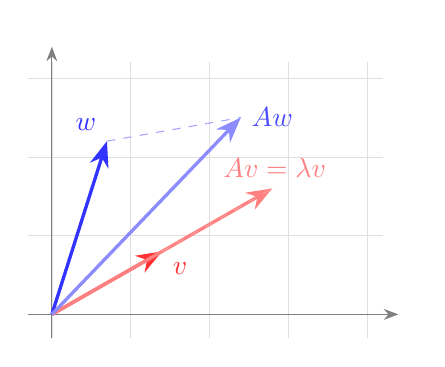
\begin{tikzpicture}[scale=1.0, >={Stealth[scale=1.1]}]
% axes
\draw[help lines, gray!25] (-0.3,-0.3) grid (4.2,3.2);
\draw[->, gray] (-0.3,0) -- (4.4,0) node[right, gray]{};
\draw[->, gray] (0,-0.3) -- (0,3.4) node[above, gray]{};
% eigen-direction: v and Av = lambda v on the SAME line
\draw[->, red!80, very thick] (0,0) -- (1.4,0.8) node[below right, red!80]{$v$};
\draw[->, red!50, very thick] (0,0) -- (2.8,1.6) node[above]{\,$Av = \lambda v$};
\draw[red!40, dashed] (1.4,0.8) -- (2.8,1.6);
% generic vector: w and Aw point in DIFFERENT directions
\draw[->, blue!80, very thick] (0,0) -- (0.7,2.2) node[above left, blue!80]{$w$};
\draw[->, blue!45, very thick] (0,0) -- (2.4,2.5) node[right, blue!70]{$Aw$};
\draw[blue!35, dashed] (0.7,2.2) -- (2.4,2.5);
\end{tikzpicture}
\end{center}

\textcolor{gray}{\small\textit{The basic idea: multiplying a vector by $A$ usually rotates \emph{and} stretches it (blue: $w \to Aw$ points elsewhere). An \textbf{eigenvector} (red) is a special direction that $A$ \emph{only stretches} -- $Av$ lies on the same line as $v$. The stretch factor is the eigenvalue $\lambda$.}}

\bigskip
\hrule
\bigskip

%% ============================================================
\subsection*{Exercise 43}
%% ============================================================

\textbf{Problem.} For $A = \begin{pmatrix} 4 & 1 & 1 \\ 2 & 5 & 2 \\ -1 & -1 & 2 \end{pmatrix}$ and $B = \begin{pmatrix} 5 & 2 & 3 \\ 2 & 4 & 2 \\ -3 & -2 & -1 \end{pmatrix}$
determine the characteristic polynomial, the eigenvalues with algebraic and geometric multiplicity, and a basis of each eigenspace -- in \textbf{two ways}.

\begin{wastun}
\begin{itemize}[leftmargin=*, nosep]
    \item \textbf{Method 1:} multiply out $\chi_A(t) = \det(A - tI)$ with the \textbf{Sarrus rule}, then factor with the \textbf{theorem on integer roots} (candidates $=$ divisors of the constant term).
    \item \textbf{Method 2:} use \textbf{row/column operations} to factor out a term $(\lambda - t)$ early -- this saves the multiplying-out.
    \item Then, per eigenvalue $\lambda$, solve the system $(A - \lambda I)v = 0$ $\Rightarrow$ basis of the eigenspace and GM.
\end{itemize}
\end{wastun}

%% --- 43 A ---
\subsubsection*{Matrix $A$}

\textbf{Method 1: Sarrus $+$ integer roots.}

\grafik

\begin{center}
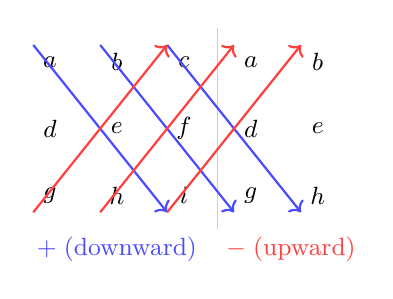
\begin{tikzpicture}[scale=0.85, every node/.style={font=\small}]
% 3x3 matrix entries plus repeated first two columns
\foreach \x/\lab in {0/a,1/b,2/c,3/a,4/b} { \node at (\x,2) {$\lab$}; }
\foreach \x/\lab in {0/d,1/e,2/f,3/d,4/e} { \node at (\x,1) {$\lab$}; }
\foreach \x/\lab in {0/g,1/h,2/i,3/g,4/h} { \node at (\x,0) {$\lab$}; }
% separator after column 3
\draw[gray!40] (2.5,-0.5) -- (2.5,2.5);
% down diagonals (+) blue
\foreach \sx in {0,1,2} {
  \draw[->, blue!70, thick] (\sx-0.25,2.25) -- (\sx+1.75,-0.25);
}
% up diagonals (-) red
\foreach \sx in {0,1,2} {
  \draw[->, red!75, thick] (\sx-0.25,-0.25) -- (\sx+1.75,2.25);
}
\node[blue!70] at (1.0,-0.8) {$+\;(\text{downward})$};
\node[red!75] at (3.6,-0.8) {$-\;(\text{upward})$};
\end{tikzpicture}
\end{center}

\textcolor{gray}{\small\textit{Sarrus rule: write the first two columns again on the right. The three diagonals going \emph{down} (blue) count $+$, the three going \emph{up} (red) count $-$. Formula: $\det = aei + bfg + cdh - ceg - afh - bdi$.}}

\textbf{Step 1: Write down $A - tI$.}
\[
A - tI = \begin{pmatrix} 4-t & 1 & 1 \\ 2 & 5-t & 2 \\ -1 & -1 & 2-t \end{pmatrix}.
\]

\textbf{Step 2: Apply Sarrus.} With the formula above (the three $+$ diagonals, then the three $-$ diagonals):
\begin{align*}
\det(A - tI) &= \underbrace{(4-t)(5-t)(2-t)}_{aei} + \underbrace{1\cdot 2 \cdot(-1)}_{bfg} + \underbrace{1\cdot 2\cdot(-1)}_{cdh} \\
&\quad - \underbrace{1\cdot(5-t)\cdot(-1)}_{ceg} - \underbrace{(4-t)\cdot 2\cdot(-1)}_{afh} - \underbrace{1\cdot 2\cdot(2-t)}_{bdi} \\[2pt]
&= (4-t)(5-t)(2-t) \;-2\;-2\;+(5-t)\;+2(4-t)\;-2(2-t).
\end{align*}
The bracket term multiplied out: $(4-t)(5-t)(2-t) = -t^3 + 11t^2 - 38t + 40$. The remaining terms: $-2 -2 +5 -t +8 -2t -4 +2t = 5 - t$. Together:
\[
\chi_A(t) = -t^3 + 11t^2 - 38t + 40 + 5 - t = -t^3 + 11t^2 - 39t + 45.
\]

\erglerk\ \textcolor{gray}{\small Quick check: constant term $\chi_A(0) = 45 = \det A$ \checkmark, and the $t^2$-coefficient $11 = \operatorname{trace}(A) = 4+5+2$ \checkmark.}

\textbf{Step 3: Factor with integer roots.} Factor out $-1$: $\chi_A(t) = -(t^3 - 11t^2 + 39t - 45)$. Integer roots divide the constant term $45$ (candidates $\pm 1, 3, 5, 9, 15, 45$). Substituting:
\[
t = 3:\; 27 - 99 + 117 - 45 = 0 \;\checkmark, \qquad t = 5:\; 125 - 275 + 195 - 45 = 0 \;\checkmark.
\]
The third root from the trace: $3 + 5 + \lambda_3 = 11 \Rightarrow \lambda_3 = 3$. So
\[
\boxed{\chi_A(t) = -(t-3)^2(t-5) = (3-t)^2(5-t).}
\]
Eigenvalues: $\lambda = 3$ (AM $2$), $\lambda = 5$ (AM $1$).

\bigskip

\textbf{Method 2: Factor out early (column trick).}

\grafik

\begin{center}
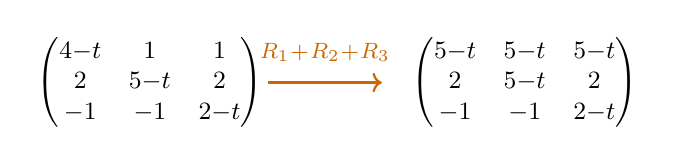
\begin{tikzpicture}[scale=0.85, every node/.style={font=\small}]
\node[anchor=west] (M) at (0,0) {$\begin{pmatrix} 4{-}t & 1 & 1 \\ 2 & 5{-}t & 2 \\ -1 & -1 & 2{-}t \end{pmatrix}$};
\draw[->, orange!80!black, thick] (3.6,0) -- (5.3,0);
\node[orange!80!black] at (4.45,0.45) {\footnotesize $R_1\!+\!R_2\!+\!R_3$};
\node[anchor=west] (R) at (5.6,0) {$\begin{pmatrix} 5{-}t & 5{-}t & 5{-}t \\ 2 & 5{-}t & 2 \\ -1 & -1 & 2{-}t \end{pmatrix}$};
\end{tikzpicture}
\end{center}

\textcolor{gray}{\small\textit{Observation: in $A$ every column sums to $5$ (e.g.\ $4+2-1 = 5$). So in $A - tI$ every column sums to $5 - t$. If you add all rows together ($R_1 \to R_1 + R_2 + R_3$), the top row becomes all $(5-t)$ -- which you can pull out as a factor.}}

\textbf{Step 1: $R_1 \to R_1 + R_2 + R_3$} (does not change the determinant), then factor out $(5-t)$:
\[
\det(A - tI) = \det\!\begin{pmatrix} 5-t & 5-t & 5-t \\ 2 & 5-t & 2 \\ -1 & -1 & 2-t \end{pmatrix}
= (5-t)\,\det\!\begin{pmatrix} 1 & 1 & 1 \\ 2 & 5-t & 2 \\ -1 & -1 & 2-t \end{pmatrix}.
\]

\textbf{Step 2: columns $C_2 \to C_2 - C_1$ and $C_3 \to C_3 - C_1$} (makes the first row $1,0,0$):
\[
= (5-t)\,\det\!\begin{pmatrix} 1 & 0 & 0 \\ 2 & 3-t & 0 \\ -1 & 0 & 3-t \end{pmatrix}
= (5-t)\,(3-t)(3-t) = (5-t)(3-t)^2.
\]

\erglerk\ \textcolor{gray}{\small The last matrix is (lower) triangular $\Rightarrow$ determinant $=$ product of the diagonal $1\cdot(3-t)\cdot(3-t)$.}

Same result as Method 1: $\chi_A(t) = (5-t)(3-t)^2$, eigenvalues $\lambda = 5$ (AM $1$), $\lambda = 3$ (AM $2$).

\medskip
\textbf{Eigenspaces.}

\textit{$\lambda = 5$:} solve $(A - 5I)v = 0$:
\[
A - 5I = \begin{pmatrix} -1 & 1 & 1 \\ 2 & 0 & 2 \\ -1 & -1 & -3 \end{pmatrix}
\xrightarrow[R_3 \to R_3 - R_1]{R_2 \to R_2 + 2R_1}
\begin{pmatrix} \piv{-1} & 1 & 1 \\ 0 & \piv{2} & 4 \\ 0 & -2 & -4 \end{pmatrix}
\xrightarrow{R_3 \to R_3 + R_2}
\begin{pmatrix} \piv{-1} & 1 & 1 \\ 0 & \piv{2} & 4 \\ 0 & 0 & 0 \end{pmatrix}.
\]
Free variable $z$: from $2y + 4z = 0 \Rightarrow y = -2z$; from $-x + y + z = 0 \Rightarrow x = y + z = -z$. With $z = 1$:
\[
E_5 = \operatorname{span}\{(-1, -2, 1)\}, \qquad \text{GM}(5) = 1.
\]

\textit{$\lambda = 3$:}
\[
A - 3I = \begin{pmatrix} 1 & 1 & 1 \\ 2 & 2 & 2 \\ -1 & -1 & -1 \end{pmatrix}
\xrightarrow[R_3 \to R_3 + R_1]{R_2 \to R_2 - 2R_1}
\begin{pmatrix} \piv{1} & 1 & 1 \\ 0 & 0 & 0 \\ 0 & 0 & 0 \end{pmatrix}.
\]
Only one equation $x + y + z = 0$, free variables $y, z$. With $(y,z) = (1,0)$ and $(0,1)$:
\[
E_3 = \operatorname{span}\{(-1, 1, 0),\, (-1, 0, 1)\}, \qquad \text{GM}(3) = 2.
\]

\[
\fbox{\parbox{0.93\textwidth}{\centering
$\chi_A(t) = (5-t)(3-t)^2$. \\[3pt]
$\lambda = 5$: AM $1$, GM $1$, basis $\{(-1,-2,1)\}$. \quad
$\lambda = 3$: AM $2$, GM $2$, basis $\{(-1,1,0),(-1,0,1)\}$. \\[3pt]
All GM $=$ AM $\Rightarrow$ $A$ is diagonalizable.
}}
\]

%% --- 43 B ---
\subsubsection*{Matrix $B$}

\textbf{Method 1: Sarrus.} With $B - tI = \begin{pmatrix} 5-t & 2 & 3 \\ 2 & 4-t & 2 \\ -3 & -2 & -1-t \end{pmatrix}$ the Sarrus rule gives (same scheme as above):
\[
\chi_B(t) = (5-t)(4-t)(-1-t) + 36 - 9t = -t^3 + 8t^2 - 20t + 16.
\]

\erglerk\ \textcolor{gray}{\small Check: $\chi_B(0) = 16 = \det B$ \checkmark, $t^2$-coefficient $8 = \operatorname{trace}(B) = 5+4-1$ \checkmark.}

\textbf{Factor:} $\chi_B(t) = -(t^3 - 8t^2 + 20t - 16)$. Test divisors of $16$: $t = 2:\; 8 - 32 + 40 - 16 = 0$ \checkmark. Polynomial division by $(t-2)$:
\[
t^3 - 8t^2 + 20t - 16 = (t-2)(t^2 - 6t + 8) = (t-2)(t-2)(t-4).
\]
\[
\boxed{\chi_B(t) = -(t-2)^2(t-4) = (2-t)^2(4-t).}
\]

\textbf{Method 2: column trick.} In $B$ too every column sums to $4$ ($5+2-3=4$, $2+4-2=4$, $3+2-1=4$). With $R_1 \to R_1+R_2+R_3$ and then $C_2 \to C_2 - C_1$, $C_3 \to C_3 - C_1$:
\[
\det(B - tI) = (4-t)\det\!\begin{pmatrix} 1 & 0 & 0 \\ 2 & 2-t & 0 \\ -3 & 1 & 2-t \end{pmatrix} = (4-t)(2-t)^2.
\]
Same result. Eigenvalues: $\lambda = 2$ (AM $2$), $\lambda = 4$ (AM $1$).

\medskip
\textbf{Eigenspaces.}

\textit{$\lambda = 4$:}
\[
B - 4I = \begin{pmatrix} 1 & 2 & 3 \\ 2 & 0 & 2 \\ -3 & -2 & -5 \end{pmatrix}
\xrightarrow[R_3 \to R_3 + 3R_1]{R_2 \to R_2 - 2R_1}
\begin{pmatrix} \piv{1} & 2 & 3 \\ 0 & \piv{-4} & -4 \\ 0 & 4 & 4 \end{pmatrix}
\xrightarrow{R_3 \to R_3 + R_2}
\begin{pmatrix} \piv{1} & 2 & 3 \\ 0 & \piv{-4} & -4 \\ 0 & 0 & 0 \end{pmatrix}.
\]
$-4y - 4z = 0 \Rightarrow y = -z$; $x + 2y + 3z = 0 \Rightarrow x = -2y - 3z = -z$. With $z=1$:
\[
E_4 = \operatorname{span}\{(-1,-1,1)\}, \qquad \text{GM}(4) = 1.
\]

\textit{$\lambda = 2$:}
\[
B - 2I = \begin{pmatrix} 3 & 2 & 3 \\ 2 & 2 & 2 \\ -3 & -2 & -3 \end{pmatrix}
\xrightarrow{R_2 \to \tfrac12 R_2}
\begin{pmatrix} 3 & 2 & 3 \\ 1 & 1 & 1 \\ -3 & -2 & -3 \end{pmatrix}
\xrightarrow[R_3 \to R_3 + 3R_2']{R_1 \to R_1 - 3R_2'}
\begin{pmatrix} 0 & -1 & 0 \\ \piv{1} & 1 & 1 \\ 0 & 1 & 0 \end{pmatrix}.
\]
From the $(-1)$ row: $-y = 0 \Rightarrow y = 0$; from $x + y + z = 0 \Rightarrow x = -z$. Only free variable $z$. With $z=1$:
\[
E_2 = \operatorname{span}\{(-1, 0, 1)\}, \qquad \text{GM}(2) = 1.
\]

\[
\fbox{\parbox{0.93\textwidth}{\centering
$\chi_B(t) = (2-t)^2(4-t)$. \\[3pt]
$\lambda = 2$: AM $2$, GM $1$, basis $\{(-1,0,1)\}$. \quad
$\lambda = 4$: AM $1$, GM $1$, basis $\{(-1,-1,1)\}$. \\[3pt]
Here GM$(2) = 1 < {}$AM$(2) = 2 \Rightarrow$ $B$ is \emph{not} diagonalizable.
}}
\]

\bigskip
\hrule
\bigskip

%% ============================================================
\subsection*{Exercise 44}
%% ============================================================

\textbf{Problem.} Determine the eigenvalues (with AM, GM) and bases of the eigenspaces of
$A = \begin{pmatrix} 1 & 0 & 5 \\ 0 & 6 & 0 \\ 1 & 0 & 5 \end{pmatrix}$ and
$B = \begin{pmatrix} 5 & 5 & 5 & 5 \\ 7 & 7 & 7 & 7 \\ 11 & 11 & 11 & 11 \\ -23 & -23 & -23 & -23 \end{pmatrix}$.

\begin{wastun}
\begin{itemize}[leftmargin=*, nosep]
    \item \textbf{No characteristic polynomial!} Instead use properties: $\lambda = 0$ exactly when $A$ is not invertible; sum of eigenvalues $= \operatorname{trace}$; product $= \det$; $\text{GM} \le \text{AM}$; read off obvious eigenvectors.
\end{itemize}
\end{wastun}

%% --- 44 A ---
\subsubsection*{Matrix $A$}

\grafik

\begin{center}
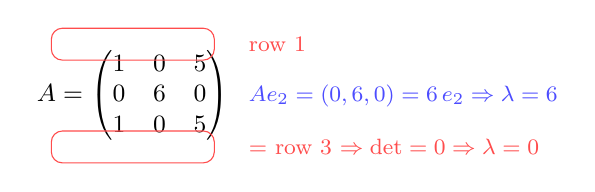
\begin{tikzpicture}[scale=0.9, every node/.style={font=\small}]
\node at (0,0) {$A = \begin{pmatrix} 1 & 0 & 5 \\ 0 & 6 & 0 \\ 1 & 0 & 5 \end{pmatrix}$};
% highlight rows 1 and 3 equal
\draw[red!70, rounded corners] (-1.15,0.5) rectangle (1.15,0.95);
\draw[red!70, rounded corners] (-1.15,-0.95) rectangle (1.15,-0.5);
\node[red!70, right] at (1.5,0.72) {\footnotesize row 1};
\node[red!70, right] at (1.5,-0.72) {\footnotesize $=$ row 3 $\Rightarrow \det = 0 \Rightarrow \lambda = 0$};
\node[blue!70, right] at (1.5,0.0) {\footnotesize $A e_2 = (0,6,0) = 6\,e_2 \Rightarrow \lambda = 6$};
\end{tikzpicture}
\end{center}

\textcolor{gray}{\small\textit{Two things are immediate: (1) row $1 =$ row $3$, so $A$ is singular $\Rightarrow$ $0$ is an eigenvalue. (2) The middle column is $(0,6,0)$, i.e.\ $A$ sends $e_2 = (0,1,0)$ to $6\,e_2$ $\Rightarrow$ $6$ is an eigenvalue with eigenvector $e_2$.}}

\textbf{Step 1: $\lambda = 0$.} Row $1 =$ row $3$ $\Rightarrow \det A = 0 \Rightarrow \lambda = 0$ is an eigenvalue. Eigenspace $= \ker A$:
\[
A v = 0:\quad 6y = 0 \Rightarrow y = 0, \qquad x + 5z = 0 \Rightarrow x = -5z.
\]
\[
E_0 = \operatorname{span}\{(-5, 0, 1)\}, \qquad \text{GM}(0) = 1.
\]

\textbf{Step 2: $\lambda = 6$.} Eigenspace $= \ker(A - 6I)$ with $A - 6I = \begin{pmatrix} -5 & 0 & 5 \\ 0 & 0 & 0 \\ 1 & 0 & -1 \end{pmatrix}$. Both nontrivial rows say $x = z$ ($y$ free). So
\[
E_6 = \operatorname{span}\{(0,1,0),\, (1,0,1)\}, \qquad \text{GM}(6) = 2.
\]

\textbf{Step 3: Add up the multiplicities.} We have $\text{GM}(6) = 2$, so $\text{AM}(6) \ge 2$. Plus $\text{AM}(0) \ge 1$. Since a $3\times 3$ matrix has exactly $3$ eigenvalues (with multiplicity), only $\text{AM}(0) = 1$, $\text{AM}(6) = 2$ remain.
\erglerk\ \textcolor{gray}{\small Check with the trace: $0\cdot 1 + 6 \cdot 2 = 12 = \operatorname{trace}(A) = 1+6+5$ \checkmark.}

\[
\fbox{\parbox{0.93\textwidth}{\centering
$\lambda = 0$: AM $1$, GM $1$, basis $\{(-5,0,1)\}$. \quad
$\lambda = 6$: AM $2$, GM $2$, basis $\{(0,1,0),(1,0,1)\}$. \\[3pt]
All GM $=$ AM $\Rightarrow$ $A$ is diagonalizable.
}}
\]

%% --- 44 B ---
\subsubsection*{Matrix $B$}

\grafik

\begin{center}
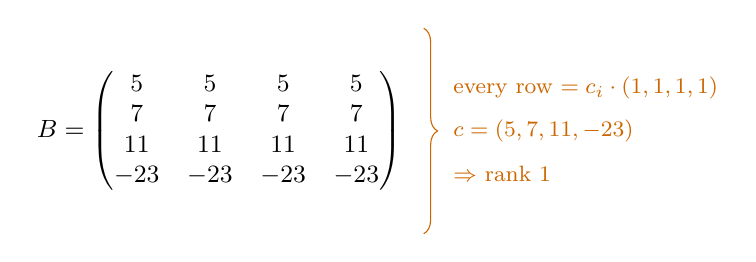
\begin{tikzpicture}[scale=0.9, every node/.style={font=\small}]
\node[anchor=west] (Bm) at (0,0) {$B = \begin{pmatrix} 5 & 5 & 5 & 5 \\ 7 & 7 & 7 & 7 \\ 11 & 11 & 11 & 11 \\ -23 & -23 & -23 & -23 \end{pmatrix}$};
\draw[decorate, decoration={brace, amplitude=5pt}, orange!80!black] ([xshift=5pt, yshift=1.45cm]Bm.east) -- ([xshift=5pt, yshift=-1.45cm]Bm.east);
\node[orange!80!black, right] at ([xshift=13pt, yshift=0.6cm]Bm.east) {\footnotesize every row $= c_i \cdot (1,1,1,1)$};
\node[orange!80!black, right] at ([xshift=13pt, yshift=0.0cm]Bm.east) {\footnotesize $c = (5,7,11,-23)$};
\node[orange!80!black, right] at ([xshift=13pt, yshift=-0.6cm]Bm.east) {\footnotesize $\Rightarrow$ rank $1$};
\end{tikzpicture}
\end{center}

\textcolor{gray}{\small\textit{$B$ has identical columns everywhere -- every row is a multiple of $(1,1,1,1)$. Such a matrix has \textbf{rank $1$}: all rows lie ``on one line''. Hence the kernel is huge (dimension $4 - 1 = 3$) and $0$ is an eigenvalue.}}

\textbf{Step 1: $\lambda = 0$ with GM $= 3$.} All columns of $B$ are equal $\Rightarrow \operatorname{rank}(B) = 1 \Rightarrow \dim\ker(B) = 4 - 1 = 3$. So $0$ is an eigenvalue with $\text{GM}(0) = 3$. The kernel: $Bv = 0$ means (each row) $5(a+b+c+d) = 0$, i.e.\ $a + b + c + d = 0$:
\[
E_0 = \operatorname{span}\{(-1,1,0,0),\, (-1,0,1,0),\, (-1,0,0,1)\}, \qquad \text{GM}(0) = 3.
\]

\textbf{Step 2: There is no further eigenvalue.} The sum of all eigenvalues $= \operatorname{trace}(B) = 5 + 7 + 11 - 23 = 0$. So far we have $\lambda = 0$ with $\text{AM}(0) \ge \text{GM}(0) = 3$. If the fourth eigenvalue $\mu$ were $\neq 0$, the sum would be $\mu \neq 0$ -- contradiction. So $\mu = 0$ and
\[
\text{AM}(0) = 4.
\]

\erglerk\ \textcolor{gray}{\small Put differently: a rank-$1$ matrix $c\,r^\top$ has only the eigenvalue $r^\top c = \operatorname{trace}$ (once) and otherwise $0$. Here $\operatorname{trace} = 0$, so \emph{all} eigenvalues are $0$ (the matrix is nilpotent, $B^2 = 0$).}

\[
\fbox{\parbox{0.93\textwidth}{\centering
$\lambda = 0$: AM $4$, GM $3$, basis $\{(-1,1,0,0),(-1,0,1,0),(-1,0,0,1)\}$. \\[3pt]
GM$(0) = 3 < {}$AM$(0) = 4 \Rightarrow$ $B$ is \emph{not} diagonalizable.
}}
\]

\bigskip
\hrule
\bigskip

%% ============================================================
\subsection*{Exercise 45}
%% ============================================================

\textbf{Problem.} $A, B \in \mathbb{F}^{n\times n}$. Prove the following claims.

\begin{wastun}
\begin{itemize}[leftmargin=*, nosep]
    \item In each claim we start with ``$\lambda$ is an eigenvalue of $A$'' $=$ ``there is $v \neq 0$ with $Av = \lambda v$'' and check that the same $v$ is also an eigenvector of the new matrix.
\end{itemize}
\end{wastun}

\textbf{(a) If $\lambda$ is an eigenvalue of $A$ and $c \in \mathbb{F}$, then $\lambda + c$ is an eigenvalue of $A + cI$.}

\textit{Proof.} Let $v \neq 0$ with $Av = \lambda v$. Then
\[
(A + cI)v = Av + c\,v = \lambda v + c v = (\lambda + c)\,v.
\]
Since $v \neq 0$, $\lambda + c$ is an eigenvalue of $A + cI$ (with the same eigenvector $v$). $\qquad\square$

\textbf{(b) If $\lambda$ is an eigenvalue of $A$, then $\lambda^2$ is an eigenvalue of $A^2$.}

\textit{Proof.} Let $v \neq 0$ with $Av = \lambda v$. Then
\[
A^2 v = A(Av) = A(\lambda v) = \lambda (Av) = \lambda (\lambda v) = \lambda^2 v. \qquad\square
\]

\textbf{(c) If $A$ is invertible and $\lambda$ is an eigenvalue of $A$, then $\lambda^{-1}$ is an eigenvalue of $A^{-1}$.}

\textit{Proof.} Since $A$ is invertible, $0$ is not an eigenvalue (otherwise there would be $v \neq 0$ with $Av = 0$, so $A$ would not be injective). Hence $\lambda \neq 0$. From $Av = \lambda v$, applying $A^{-1}$:
\[
v = A^{-1}(\lambda v) = \lambda\, A^{-1} v \;\Longrightarrow\; A^{-1} v = \tfrac{1}{\lambda}\, v.
\]
Since $v \neq 0$, $\lambda^{-1}$ is an eigenvalue of $A^{-1}$. $\qquad\square$

\textbf{(d) If $v$ is an eigenvector of both $A$ and $B$, then $v$ is also an eigenvector of $AB$.}

\textit{Proof.} Let $v \neq 0$ with $Av = \lambda v$ and $Bv = \mu v$. Then
\[
(AB)v = A(Bv) = A(\mu v) = \mu (Av) = \mu (\lambda v) = (\lambda\mu)\,v.
\]
Since $v \neq 0$, $v$ is an eigenvector of $AB$ for the eigenvalue $\lambda\mu$. $\qquad\square$

\bigskip
\hrule
\bigskip

%% ============================================================
\subsection*{Overview: Results 43 \& 44}
%% ============================================================

\begin{center}
\begin{tabular}{@{}llll@{}}
\toprule
Matrix & Eigenvalue ($\lambda$) & AM, GM & Basis of the eigenspace \\
\midrule
$43\,A$ & $3$ & $2,\,2$ & $(-1,1,0),\,(-1,0,1)$ \\
        & $5$ & $1,\,1$ & $(-1,-2,1)$ \\[2pt]
$43\,B$ & $2$ & $2,\,1$ & $(-1,0,1)$ \\
        & $4$ & $1,\,1$ & $(-1,-1,1)$ \\[2pt]
$44\,A$ & $0$ & $1,\,1$ & $(-5,0,1)$ \\
        & $6$ & $2,\,2$ & $(0,1,0),\,(1,0,1)$ \\[2pt]
$44\,B$ & $0$ & $4,\,3$ & $(-1,1,0,0),\,(-1,0,1,0),\,(-1,0,0,1)$ \\
\bottomrule
\end{tabular}
\end{center}

\textit{Diagonalizable} are $43\,A$ and $44\,A$ (all GM $=$ AM). \emph{Not} diagonalizable are $43\,B$ and $44\,B$ (one GM $<$ AM each).

\end{document}
